% !TEX root = ../BookTemplate.tex
%%%%%%%%%%%%%%%%%%%%%%%%%%%%%%%%%%%%%%%%%%%%%%%%%%%%%%%%%%%%%%%%%%%%%%%%%%%%
\chapter{TD-PINNs: Time-Discrete Physics-Informed Neural Networks
         Applied to the Viscous Burgers Equation}

% ─────────────────────────────────────────────────────────────────────────────
\section*{Introduction}
% ─────────────────────────────────────────────────────────────────────────────

Physics-Informed Neural Networks (PINNs), introduced by Raissi et
al.~\cite{Raissi2019}, embed the residual of a partial differential equation
directly into the training loss, which makes it possible to solve forward and
inverse problems without a mesh and without labelled data. This flexibility
comes at a price: because a vanilla PINN approximates the entire space--time
domain with a single network, it struggles to converge on time-dependent
problems with stiff or strongly nonlinear dynamics~\cite{Krishnapriyan2021}.

Time-Discrete Physics-Informed Neural Networks (TD-PINNs) sidestep this
difficulty by splitting the global problem into a sequence of purely spatial
subproblems---one per time step---each solved by an independent network that
inherits its predecessor's solution as a frozen input. Sanabria
\citeyear{pipe} demonstrated the idea on a simple diffusion case with an
explicit Euler discretisation. This chapter builds on that baseline in two
ways. We first add a Backward Euler (implicit) scheme, which is
unconditionally stable and therefore removes the CFL restriction on the time
step; we then introduce a Crank--Nicholson scheme, which recovers second-order
temporal accuracy while keeping that unconditional stability. Both schemes are
new relative to Sanabria's \citeyear{pipe} explicit-only formulation. We
validate the framework on the viscous Burgers equation against the Hopf--Cole
sawtooth analytic solution, and we compare five collocation-point strategies
head to head.

% ─────────────────────────────────────────────────────────────────────────────
\section{Background and Related Work}
% ─────────────────────────────────────────────────────────────────────────────

\subsection{Physics-Informed Neural Networks}

The PINN framework~\cite{Raissi2019} trains a network
$\hat{u}(x,t;\theta)$ by minimising a composite loss that penalises the PDE
residual together with the misfit of the initial and boundary conditions. For
a general time-dependent PDE $\mathcal{N}[u] = 0$, the loss reads
\[
  \mathcal{L}(\theta)
  = \lambda_\text{PDE}\,\mathcal{L}_\text{PDE}
  + \lambda_\text{IC}\,\mathcal{L}_\text{IC}
  + \lambda_\text{BC}\,\mathcal{L}_\text{BC},
\]
where each term is a mean-squared residual evaluated at a finite set of
collocation points. A well-known difficulty is that the weights $\lambda$ have
no natural scale: their magnitudes depend on the problem, and a poor choice
lets one component dominate training and starve the
others~\cite{Wang2021}. Adaptive weighting based on the Neural Tangent Kernel
(NTK) has been proposed to relieve this pathology~\cite{Wang2021}.

\subsection{Collocation Point Strategies}

Where the collocation points are placed strongly affects convergence. Pure
random (Monte Carlo) sampling is simple but wasteful when the solution has
localised features. Lu et al.~\cite{Lu2019} proposed residual-based adaptive
refinement (RAR), which adds points in high-residual regions during training,
while McClenny and Braga-Neto~\cite{McClenny2021} introduced self-adaptive
weights that assign a per-point importance during the optimisation and so
concentrate effort near difficult regions. More recently, Chiu et
al.~\cite{Chiu2022} coupled automatic differentiation with finite-difference
stencils at the collocation points (can-PINN); by tightly linking neighbouring
locations, this improves accuracy by one to two orders of magnitude over
standard AD-based PINNs, especially in the sparse-sampling regime where vanilla
PINNs otherwise converge to unphysical solutions.

\subsection{Time-Discrete and Time-Marching PINNs}

Raissi et al.~\cite{Raissi2019} already introduced discrete-time PINNs based on
implicit Runge--Kutta schemes with an arbitrarily large number of stages,
which enables very large time steps. That approach, however, takes a single
large leap rather than many small steps, which limits its use for multi-step
dynamics. Later work showed that standard PINNs can fail outright on
convection-dominated problems because of non-convex loss landscapes, and that
curriculum learning or time-marching are necessary
remedies~\cite{Krishnapriyan2021,Daw2023}. Chen et al.~\cite{Chen2023} and
Gómez-Barrera~\cite{pipe} independently showed that pairing backward Euler or
Crank--Nicholson time-stepping with a sequence of single-network spatial
problems (TL-DPINN and TD-PINN, respectively) yields stable and accurate
solutions; the TL-DPINN study found that Crank--Nicholson strikes the best
balance between cost and accuracy among the first- and second-order implicit
schemes. Bravo et al.~\cite{Bravo2024} extended step-by-step TD-PINNs to
implicit and implicit--explicit schemes on stiff sustainability models,
confirming both the stability advantage of backward Euler and the precision
advantage of Crank--Nicholson.

\subsection{Spectral Bias in PINNs}

A structural limitation of MLP-based PINNs is \emph{spectral bias} (the
F-Principle): networks with smooth activations ($\tanh$, $\sin$, ReLU) learn
the low-frequency components of the solution first and need many more
iterations or collocation points to resolve high-frequency
features~\cite{Rahaman2019}. For Burgers' equation at low viscosity this shows
up as under-resolved sharp gradients. Wang et al.~\cite{Wang2021} traced the
bias to the eigenspectrum of the Neural Tangent Kernel: the gradient of the
PDE loss dominates those of the IC and BC losses by orders of magnitude,
producing imbalanced training dynamics that are especially damaging when the
solution has multi-scale spatial structure.

% ─────────────────────────────────────────────────────────────────────────────
\section{Burgers Equation and Analytic Benchmark}
% ─────────────────────────────────────────────────────────────────────────────

The one-dimensional viscous Burgers equation is
\begin{equation}
  \frac{\partial u}{\partial t}
  + u\,\frac{\partial u}{\partial x}
  = \nu\,\frac{\partial^2 u}{\partial x^2},
  \qquad x \in [0, 2\pi],\quad t \in [0, T],
  \label{eq:burgers}
\end{equation}
where $u = u(x,t)$ is the velocity field and $\nu > 0$ is the kinematic
viscosity. The nonlinear advection term $u\,\partial u/\partial x$ steepens
wave fronts while the diffusion term $\nu\,\partial^2 u/\partial x^2$
regularises them. Burgers' equation is among the most representative
benchmarks in computational fluid dynamics precisely because it captures both
mechanisms at once, mirroring the structure of the Navier--Stokes equations in
one dimension.

\subsection{Hopf--Cole Sawtooth Analytic Solution}

The Hopf--Cole transformation maps Burgers' equation onto the heat equation
and yields an exact closed-form solution. For the sawtooth initial profile on
$[0,2\pi]$ it reads
\begin{equation}
  u(x,t)
  = 2\nu\,\frac{\partial_x \phi}{\phi} + 4,
  \qquad
  \phi = e^{-a} + e^{-b},
  \label{eq:hopf_cole}
\end{equation}
with
\[
  a = \frac{(x - 4t)^2}{4\nu(t+1)},
  \qquad
  b = \frac{(x - 4t - 2\pi)^2}{4\nu(t+1)}.
\]
This analytic solution plays a dual role: it defines the initial condition
$u(x,0)$ handed to the first network, and it provides the ground truth against
which every numerical error in this chapter is measured.

\begin{Rmk}{Well-posedness of the benchmark}{rmk:benchmark}
  For $\nu = 0.07$ and $T = 0.025$ the profile stays well-resolved throughout
  the simulation window: its gradients are steep enough to challenge the
  collocation strategies, yet no true discontinuity forms within $[0,T]$. This
  makes the case tractable but non-trivial.
\end{Rmk}

% ─────────────────────────────────────────────────────────────────────────────
\section{Time Discretisation Schemes}
% ─────────────────────────────────────────────────────────────────────────────

\subsection{TD-PINN Computation Graph}

The computation performed at each time level is summarised in
Figure~\ref{fig:tdpinn_diagram}. The network $u^{t-1}$ trained at the previous
step is frozen: its output and spatial derivatives are evaluated once and
stored as constants. The current network $u^t$ takes the spatial coordinate
$x$ as input and is optimised by minimising the total loss $\mathcal{L}$, with
all of its derivatives obtained by automatic differentiation (AD). Once
training converges, $u^t$ takes over the frozen role and the cycle advances to
$u^{t+1}$.

\begin{figure}[H]
\centering
\resizebox{\textwidth}{!}{%
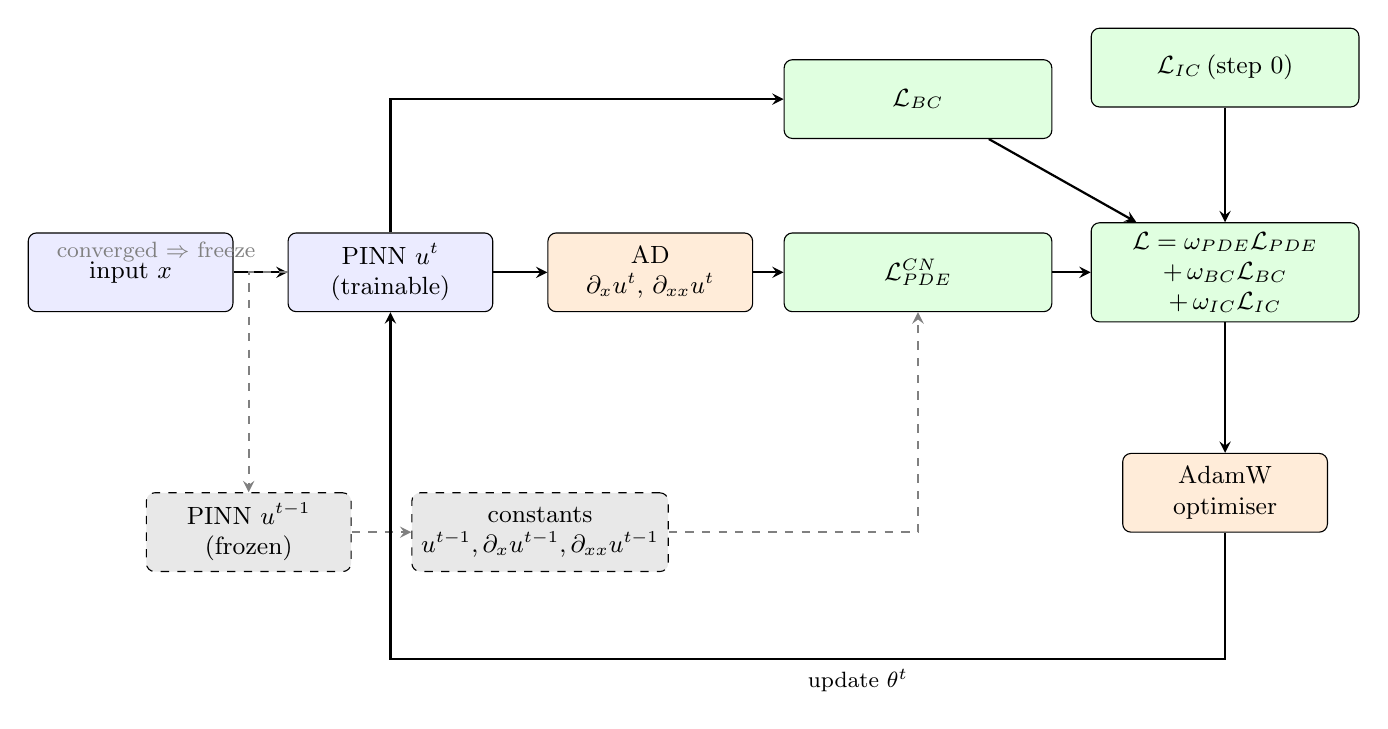
\begin{tikzpicture}[
    every node/.style = {font=\small},
    box/.style     = {draw, rounded corners=3pt, minimum width=2.6cm,
                      minimum height=1.0cm, align=center, fill=blue!8},
    frozen/.style  = {draw, rounded corners=3pt, minimum width=2.6cm,
                      minimum height=1.0cm, align=center, fill=gray!18, dashed},
    compute/.style = {draw, rounded corners=3pt, minimum width=2.6cm,
                      minimum height=1.0cm, align=center, fill=orange!15},
    loss/.style    = {draw, rounded corners=3pt, minimum width=3.4cm,
                      minimum height=1.0cm, align=center, fill=green!12},
    arrow/.style   = {-stealth, thick},
    darrow/.style  = {-stealth, thick, dashed, gray},
  ]

  %% main current-network flow (top line, y = 0)
  \node[box]     (input) at (0,0)      {input $x$};
  \node[box]     (curr)  at (3.3,0)    {PINN $u^{t}$\\(trainable)};
  \node[compute] (ad)    at (6.6,0)    {AD\\$\partial_x u^{t},\,\partial_{xx} u^{t}$};
  \node[loss]    (lpde)  at (10.0,0)   {$\mathcal{L}_\text{PDE}^{\text{CN}}$};
  \node[loss]    (ltot)  at (13.9,0)
        {$\mathcal{L}=\omega_\text{PDE}\mathcal{L}_\text{PDE}$\\
         $+\,\omega_\text{BC}\mathcal{L}_\text{BC}$\\
         $+\,\omega_\text{IC}\mathcal{L}_\text{IC}$};

  %% auxiliary loss terms
  \node[loss] (lbc) at (10.0, 2.2)  {$\mathcal{L}_\text{BC}$};
  \node[loss] (lic) at (13.9, 2.6)  {$\mathcal{L}_\text{IC}$\,(step 0)};

  %% optimiser
  \node[compute] (opt) at (13.9,-2.8) {AdamW\\optimiser};

  %% frozen previous-step branch (bottom line, y = -3.3)
  \node[frozen] (prev)  at (1.5,-3.3) {PINN $u^{t-1}$\\(frozen)};
  \node[frozen] (grads) at (5.2,-3.3)
        {constants\\$u^{t-1},\partial_x u^{t-1},\partial_{xx}u^{t-1}$};

  %% ── flow arrows ──────────────────────────────────────────────────────
  \draw[arrow]  (input) -- (curr);
  \draw[arrow]  (curr)  -- (ad);
  \draw[arrow]  (ad)    -- (lpde);
  \draw[arrow]  (lpde)  -- (ltot);
  \draw[arrow]  (curr.north) |- (lbc.west);
  \draw[arrow]  (lbc) -- (ltot);
  \draw[arrow]  (lic) -- (ltot);
  \draw[arrow]  (ltot) -- (opt);

  %% frozen branch
  \draw[darrow] (prev) -- (grads);
  \draw[darrow] (grads.east) -| (lpde.south);

  %% feedback: optimiser updates the current network (along the bottom)
  \draw[arrow]  (opt.south) -- ++(0,-1.6)
        -| node[pos=0.22, below, font=\footnotesize]{update $\theta^t$}
        (curr.south);

  %% step completion: freeze the current network
  \draw[darrow] (curr.west) -|
        node[pos=0.28, above left, font=\footnotesize]{converged $\Rightarrow$ freeze}
        (prev.north);

\end{tikzpicture}}
\caption{TD-PINN computation graph at step $t$ (Crank--Nicholson). Dashed grey
  boxes and arrows are frozen, no-grad quantities inherited from step $t{-}1$;
  solid arrows are computed by automatic differentiation on the current
  network.}
\label{fig:tdpinn_diagram}
\end{figure}

\subsection{Explicit Euler --- Baseline \texorpdfstring{\protect\citep{pipe}}{(Sanabria)}}

Sanabria \citeyear{pipe} demonstrated the TD-PINN concept on a pure diffusion
equation with explicit Euler time discretisation. There, every spatial
operator is evaluated at the \emph{known} level $t$,
\[
  \frac{u^{t+1} - u^{t}}{\Delta t}
  = \nu\left[\frac{\partial^2 u}{\partial x^2}\right]^{\!t},
\]
so the right-hand side is read off the already-trained network $u^t$ (frozen
parameters) and training $u^{t+1}$ collapses to a supervised regression. The
price is conditional stability.

\begin{Rmk}{Conditional stability}{rmk:cfl}
  The explicit scheme is only conditionally stable: the CFL condition
  $\Delta t \leq (\Delta x)^2/(2\nu)$ forces very small time steps on fine
  grids or at low viscosity. In its original form it was applied to diffusion
  only; here it is extended to the full nonlinear Burgers equation.
\end{Rmk}

\subsection{Implicit Euler --- Unconditional Stability}

Evaluating every PDE term at the \emph{unknown} level $t$ instead gives the
Backward Euler scheme,
\[
  \frac{u^{t} - u^{t-1}}{\Delta t}
  + u^{t}\left[\frac{\partial u^{t}}{\partial x}\right]
  = \nu\left[\frac{\partial^2 u^{t}}{\partial x^2}\right],
\]
where $u^{t-1}$ is the previously trained network (frozen, treated as a
constant) and the derivatives of $u^t$ come from automatic differentiation on
the network currently being trained. Rearranged, the PDE loss at step $t$ is
\begin{equation}
  \mathcal{L}_\text{PDE}^{\text{BE}}
  = \left\langle\left(
      \frac{u^{t} - u^{t-1}}{\Delta t}
      + u^{t}\frac{\partial u^{t}}{\partial x}
      - \nu\frac{\partial^2 u^{t}}{\partial x^2}
    \right)^{\!2}\right\rangle_{\!\mathcal{X}},
  \label{eq:loss_be}
\end{equation}
with $\langle\cdot\rangle_{\mathcal{X}}$ the mean over the collocation set.
Unlike the explicit case, this loss imposes no relation between $\Delta t$ and
$\Delta x$, so the scheme is unconditionally stable; its truncation error is
$\mathcal{O}(\Delta t)$, in agreement with the TL-DPINN~\cite{Chen2023} and
step-by-step TD-PINN~\cite{Bravo2024} results.

\subsection{Crank--Nicholson --- Second-Order Accuracy}

Backward Euler is only first-order accurate in time. Crank--Nicholson recovers
$\mathcal{O}(\Delta t^2)$ accuracy by averaging the spatial residual at levels
$t-1$ and $t$:
\begin{equation}
  \frac{u^{t} - u^{t-1}}{\Delta t}
  = \frac{1}{2}\Bigg[
      \underbrace{\left(
        \nu\!\left[\frac{\partial^2 u}{\partial x^2}\right]^{\!t-1}
        - u\!\left[\frac{\partial u}{\partial x}\right]^{\!t-1}
      \right)}_{\text{from PINN }t{-}1\ (\text{frozen})}
      +
      \underbrace{\left(
        \nu\!\left[\frac{\partial^2 u}{\partial x^2}\right]^{\!t}
        - u\!\left[\frac{\partial u}{\partial x}\right]^{\!t}
      \right)}_{\text{from PINN }t\ (\text{AD})}
    \Bigg].
  \label{eq:cn_scheme}
\end{equation}
The level-$(t-1)$ terms are extracted from the previously trained network: its
values and spatial derivatives are computed once at the end of step $t-1$ and
stored as fixed tensors, so no backpropagation through the old network is
needed during the current step. The level-$t$ terms are differentiated by AD.
The resulting PDE loss is
\begin{equation}
  \mathcal{L}_\text{PDE}^{\text{CN}}
  = \left\langle\left(
      \frac{u^{t} - u^{t-1}}{\Delta t}
      - \frac{1}{2}\!\left[
          \nu\frac{\partial^2 u^{t-1}}{\partial x^2}
          - u^{t-1}\frac{\partial u^{t-1}}{\partial x}
          + \nu\frac{\partial^2 u^{t}}{\partial x^2}
          - u^{t}\frac{\partial u^{t}}{\partial x}
        \right]
    \right)^{\!2}\right\rangle_{\!\mathcal{X}}.
  \label{eq:loss_cn}
\end{equation}

% ─────────────────────────────────────────────────────────────────────────────
\section{Boundary Conditions and Total Loss}
\label{sec:bc}
% ─────────────────────────────────────────────────────────────────────────────

The network at step $t$ is trained on a total loss that combines three terms,
\begin{equation}
  \mathcal{L}
  = \omega_\text{PDE}\,\mathcal{L}_\text{PDE}
  + \omega_\text{BC}\,\mathcal{L}_\text{BC}
  + \omega_\text{IC}\,\mathcal{L}_\text{IC},
  \label{eq:total_loss}
\end{equation}
with scalar weights $\omega_\text{PDE}, \omega_\text{BC}, \omega_\text{IC}
\geq 0$. Only $\mathcal{L}_\text{IC}$ is active at the initial step ($t=0$); at
every later step only $\mathcal{L}_\text{PDE}$ and $\mathcal{L}_\text{BC}$
remain.

\paragraph{Boundary-condition loss.}
For periodic or homogeneous Dirichlet conditions at $x \in \{0,\,2\pi\}$,
\[
  \mathcal{L}_\text{BC}
  = \frac{1}{N_\text{BC}}\sum_{j=1}^{N_\text{BC}}
    \bigl(u^t(x_j^\text{BC}) - u_\text{BC}(x_j)\bigr)^2 .
\]

\paragraph{Initial-condition loss.}
At $t=0$ the network is fitted directly to the analytic Hopf--Cole profile,
\[
  \mathcal{L}_\text{IC}
  = \frac{1}{N_\text{IC}}\sum_{i=1}^{N_\text{IC}}
    \bigl(u^0(x_i) - u_0(x_i)\bigr)^2,
  \qquad u_0(x) = u(x,0)\big|_{\text{Hopf--Cole}} .
\]

\begin{Rmk}{Limitation of scalar weights}{rmk:weights}
  The weights $\omega$ in \eqref{eq:total_loss} have no natural metric
  interpretation: the magnitudes of $\mathcal{L}_\text{PDE}$,
  $\mathcal{L}_\text{BC}$, and $\mathcal{L}_\text{IC}$ are heterogeneous and
  problem-scale-dependent, so choosing $\omega$ is partly arbitrary and a poor
  choice lets one term dominate and the others be ignored~\cite{Wang2021}.
  Hard-constraint formulations such as the augmented-Lagrangian approach of
  Sukumar and Srivastava~\cite{Sukumar2022} or the NTK-based annealing of Wang
  et al.~\cite{Wang2021} partly alleviate this.
\end{Rmk}

% ─────────────────────────────────────────────────────────────────────────────
\section{Collocation Point Strategies}
% ─────────────────────────────────────────────────────────────────────────────

The collocation set $\mathcal{X} = \{x_i\}_{i=1}^{N}$ fixes where the PDE loss
is evaluated during training. We implement five strategies. To preserve global
coverage, every non-uniform strategy complements its $N_\text{adapt}$ selected
points with $N_\text{unif}$ uniformly sampled ones:
\begin{equation}
  N = N_\text{adapt} + N_\text{unif}
    = \alpha \cdot N_\text{total} + \beta \cdot N_\text{total},
  \quad \alpha + \beta = 1.
  \label{eq:split}
\end{equation}

\begin{De}{Collocation strategies}{de:collocation}
The five strategies implemented in this work are:
\begin{description}
  \item[\boxlabel{Uniform}{1.8cm}]
    Points drawn independently from $\mathcal{U}(x_\min, x_\max)$.

  \item[\boxlabel{LHS-1D}{1.8cm}]
    Latin Hypercube Sampling: the domain is split into $N$ equal bins with one
    point per bin~\cite{Lu2019}.

  \item[\boxlabel{Gradient}{1.8cm}]
    Top-$N_\text{adapt}$ points by $|\partial u^t/\partial x|$, filled to $N$
    with uniform samples via Eq.~\eqref{eq:split}.

  \item[\boxlabel{Curvature}{1.8cm}]
    Top-$N_\text{adapt}$ points by $|\partial^2 u^t/\partial x^2|$, filled
    analogously.

  \item[\boxlabel{Residual}{1.8cm}]
    Top-$N_\text{adapt}$ points by $|\mathrm{LF}(x)|$ inherited from
    $\mathcal{X}^{t-1}$, filled uniformly. Two variants:
    \textit{last\_residual} (final epoch of step $t{-}1$) and
    \textit{mean\_residual} (epoch average). Related to RAR~\cite{Lu2019} and
    SA-PINNs~\cite{McClenny2021}.
\end{description}
\end{De}

% ─────────────────────────────────────────────────────────────────────────────
\subsection{Pure Diffusion Benchmark}
\label{subsec:colloc_diffusion}
% ─────────────────────────────────────────────────────────────────────────────

We first test the strategies on the pure diffusion equation with a Gaussian
initial condition, a controlled and operator-simple setting that isolates the
sampling question before the nonlinear Burgers case:
\begin{equation}
  \frac{\partial u}{\partial t} = \nu\,\frac{\partial^2 u}{\partial x^2},
  \qquad x \in [0,2\pi],\quad t \in [0,T],\quad \nu = 2,
  \label{eq:diffusion}
\end{equation}
with homogeneous Dirichlet conditions $u(0,t) = u(2\pi,t) = 0$ and a Gaussian
initial profile centred at $x_c = \pi$ of width $\sigma_0 = 0.5$, namely
$u(x,0) = \exp\!\left(-(x-\pi)^2/2\sigma_0^2\right)$. The heat-kernel
convolution gives the exact solution, a Gaussian that spreads and decays while
keeping its shape (Figure~\ref{fig:diffusion_heatkernel}),
\begin{equation}
  u(x,t) = \frac{\sigma_0}{\sqrt{\sigma_0^2 + 2\nu t}}
    \exp\!\left(-\frac{(x-x_c)^2}{2(\sigma_0^2 + 2\nu t)}\right),
  \label{eq:diffusion_exact}
\end{equation}
whose effective variance $\sigma^2(t) = \sigma_0^2 + 2\nu t$ grows linearly in
time. The amplitude decays as $1/\sqrt{\sigma^2(t)}$ to conserve the $L^1$ norm
(total ``mass''), while the peak curvature
$|\partial^2 u/\partial x^2|_\text{max} \propto \sigma^{-2}(t)$ falls
monotonically yet stays concentrated near the peak at all times.

\begin{figure}[H]
  \centering
  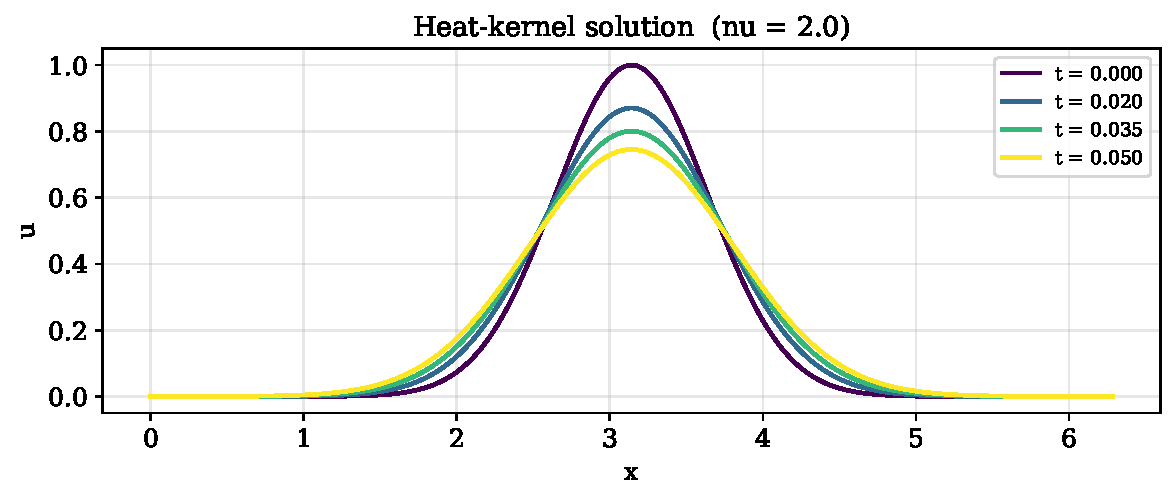
\includegraphics[width=0.72\textwidth]{figs/diffussion_heat_kernel.pdf}
  \caption{Heat-kernel solution \eqref{eq:diffusion_exact} at
    $t \in \{0,\,0.02,\,0.035,\,0.05\}$ ($\nu = 2$, $\sigma_0 = 0.5$).}
  \label{fig:diffusion_heatkernel}
\end{figure}

Because the exact solution is a smooth, unimodal profile, its single dominant
feature is captured entirely by the second derivative: the curvature
$|\partial^2 u/\partial x^2|$ follows the amplitude envelope of the diffusing
Gaussian and peaks exactly where the PDE residual is largest. Curvature-based
sampling therefore places points precisely where the network struggles most,
which gives it a structural edge over the other strategies on this problem, and
the numerics in Figure~\ref{fig:colloc_diffusion_errors} bear this out. Across
all three norms the curvature criterion attains the lowest mean error
(mean $L^1 = 4.54\times10^{-2}$, mean $L^2 = 1.96\times10^{-2}$), edging out
uniform ($L^1 = 4.72\times10^{-2}$), LHS ($4.69\times10^{-2}$), and gradient
($4.74\times10^{-2}$). The separation is clearest in the worst-case $L^\infty$
norm, where curvature yields the smallest peak error at every time level
because the Gaussian's single active feature is always tracked. The
residual-based strategies reach competitive accuracy but at a much higher epoch
cost (Figure~\ref{fig:colloc_diffusion_epochs}: ${\sim}55\,000$ epochs versus
${\sim}8\,000$ for curvature, roughly $7\times$ more), since they must first
evaluate the previous step's residual before they can adapt.

\begin{figure}[H]
  \centering
  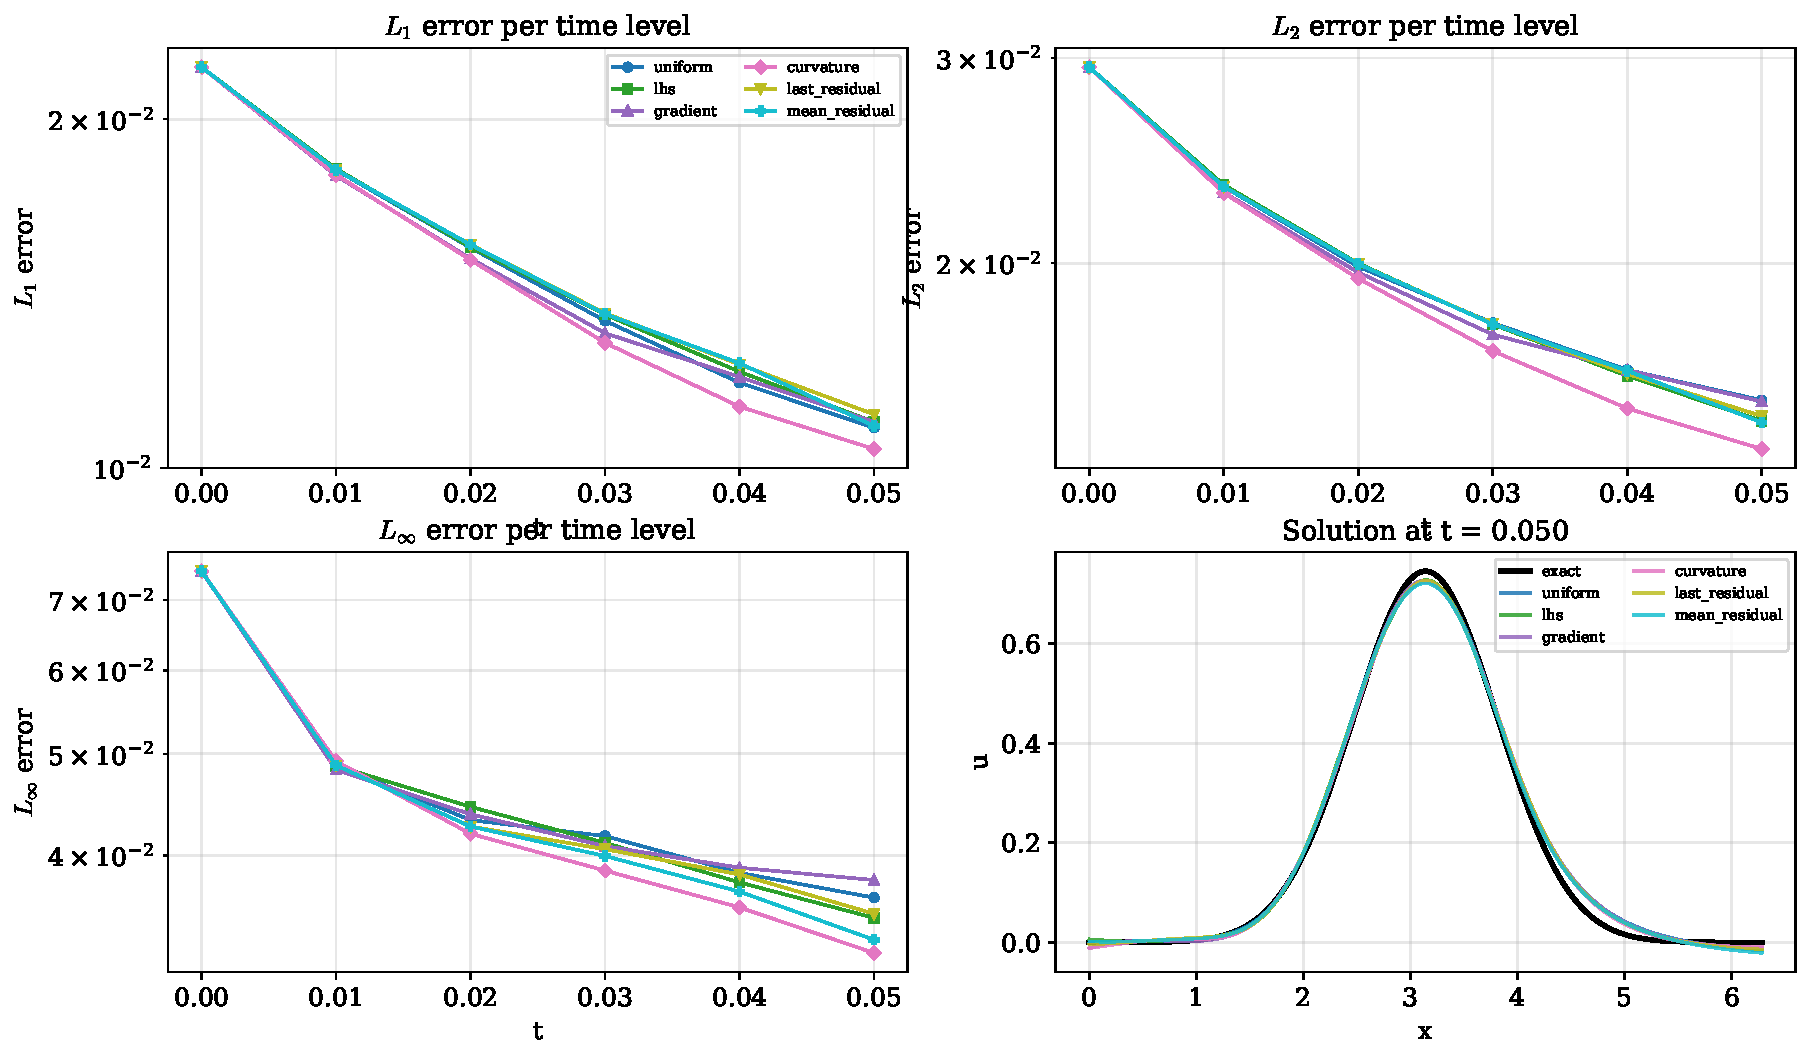
\includegraphics[width=\textwidth]{figs/collocation_diffusion_errors.pdf}
  \caption{Collocation comparison on the diffusion equation
    \eqref{eq:diffusion}: $L^1$, $L^2$, and $L^\infty$ errors per time level,
    and solution profiles at $t = 0.05$.}
  \label{fig:colloc_diffusion_errors}
\end{figure}

\begin{figure}[H]
  \centering
  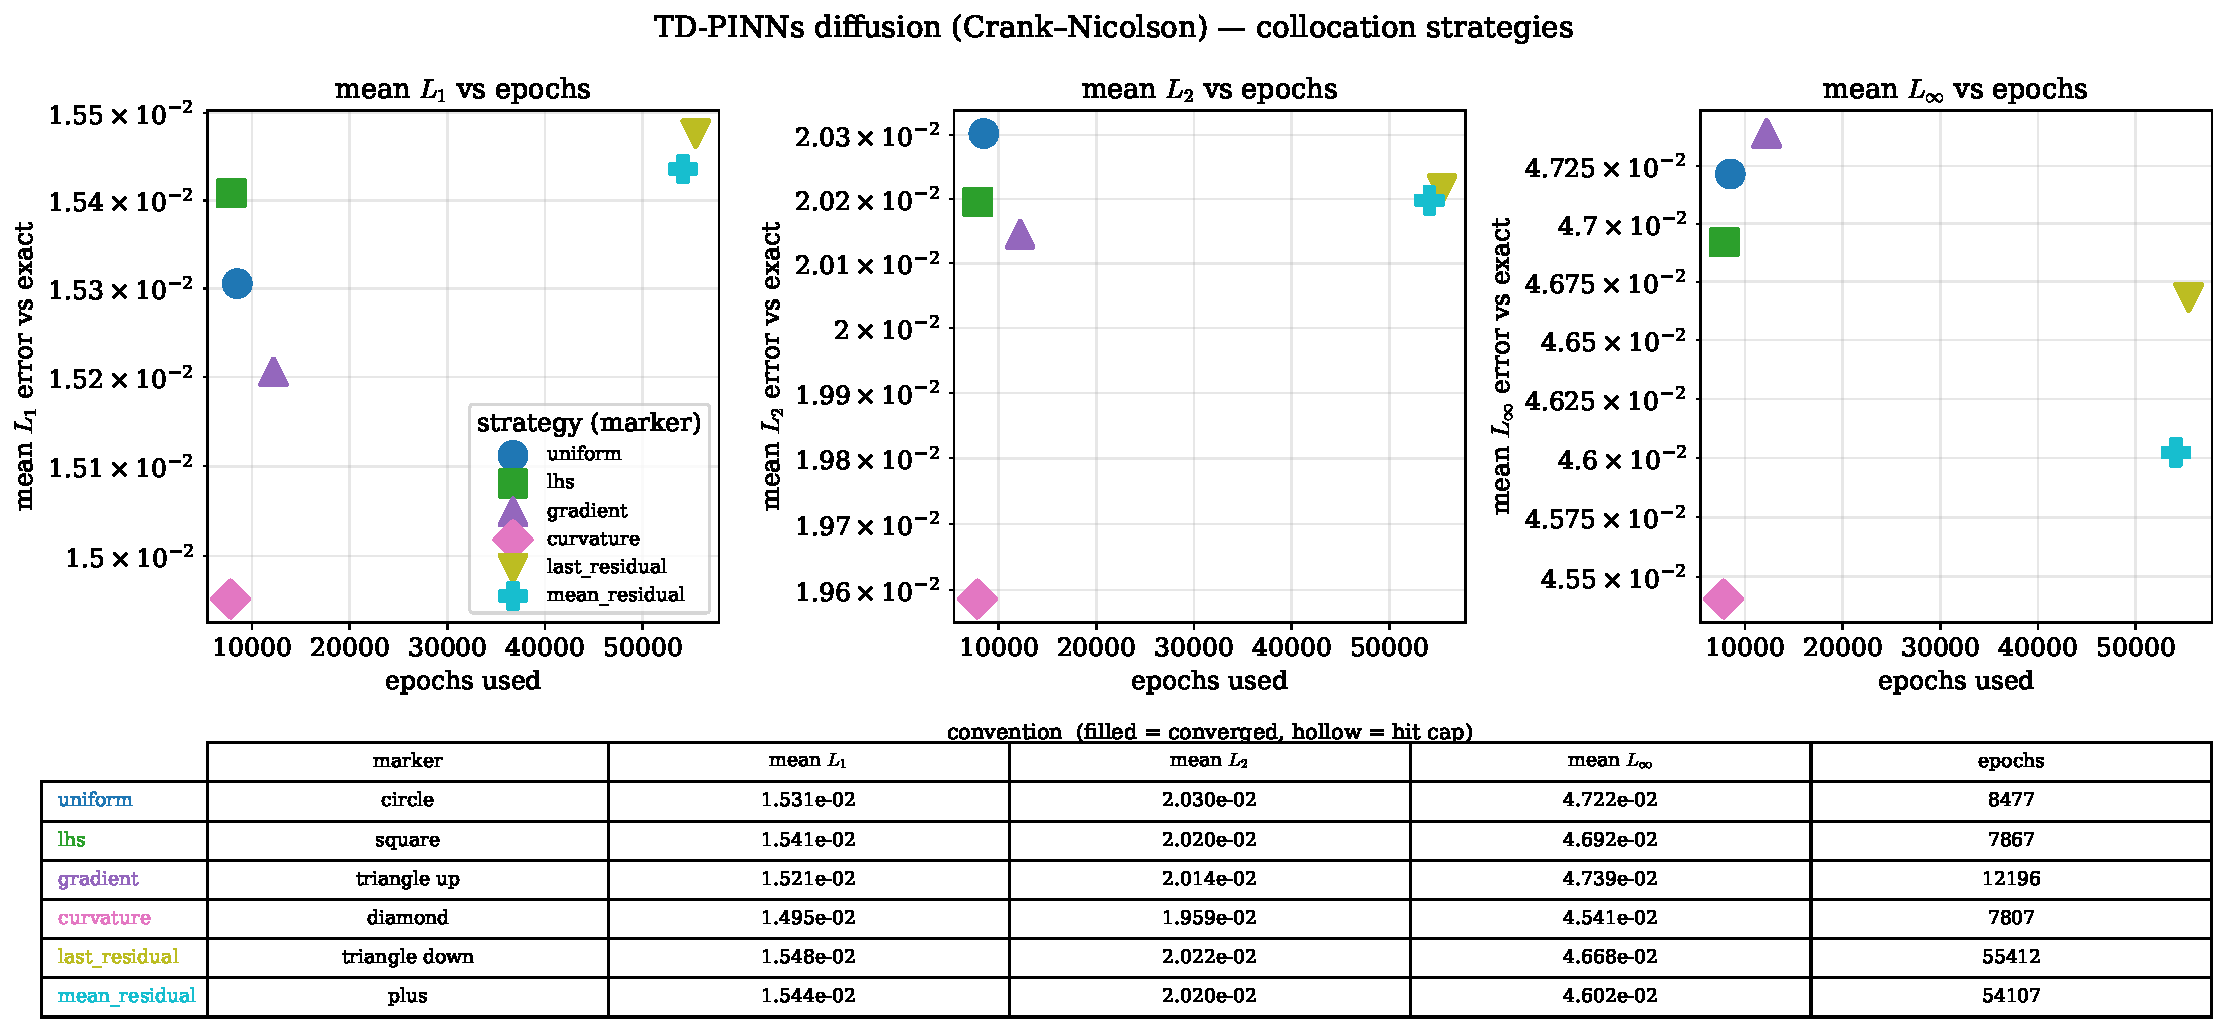
\includegraphics[width=0.75\textwidth]{figs/collocation_diffusion_epochs_norms.pdf}
  \caption{Mean error versus total epoch count for the diffusion problem.}
  \label{fig:colloc_diffusion_epochs}
\end{figure}

% ─────────────────────────────────────────────────────────────────────────────
\subsection{Burgers' Equation: the Nonlinear Case}
\label{subsec:colloc_burgers}
% ─────────────────────────────────────────────────────────────────────────────

The picture changes for Burgers' equation. The advection term
$u\,\partial u/\partial x$ couples all spatial scales, so regions of high
gradient and high curvature shift and interact over time and no single
physics-derived criterion consistently flags the most informative locations.
Gradient- and curvature-based sampling over-concentrate points around the
dominant feature of the \emph{current} step and neglect the background region
into which the solution is about to evolve. What works instead is to measure
directly where the network is currently wrong: residual-based sampling selects
the points where the PDE residual $|\mathrm{LF}(x)|$ was largest at the end of
the previous step, a model-free proxy for the error landscape that assumes
nothing about which operator dominates.

Figures~\ref{fig:colloc_burgers_sol} and \ref{fig:colloc_burgers_epochs}
confirm this ordering. In mean $L^1$ error, \textit{mean\_residual} reaches
$0.480$ and \textit{last\_residual} $0.481$, both slightly better than uniform
($0.482$), gradient ($0.482$), and curvature ($0.482$). LHS matches that
accuracy level ($0.485$) at a dramatically lower epoch cost
($16\,427$ epochs versus $142\,000$--$276\,000$ for the physics-derived
strategies). The solution profiles at $t = 0.025$ show every strategy tracking
the sawtooth closely, with the error falling from $L^\infty \approx 0.63$ at the
first step to $L^\infty \approx 0.24$ at the last; the network therefore
improves systematically as the solution broadens and its gradients relax.

\begin{figure}[H]
  \centering
  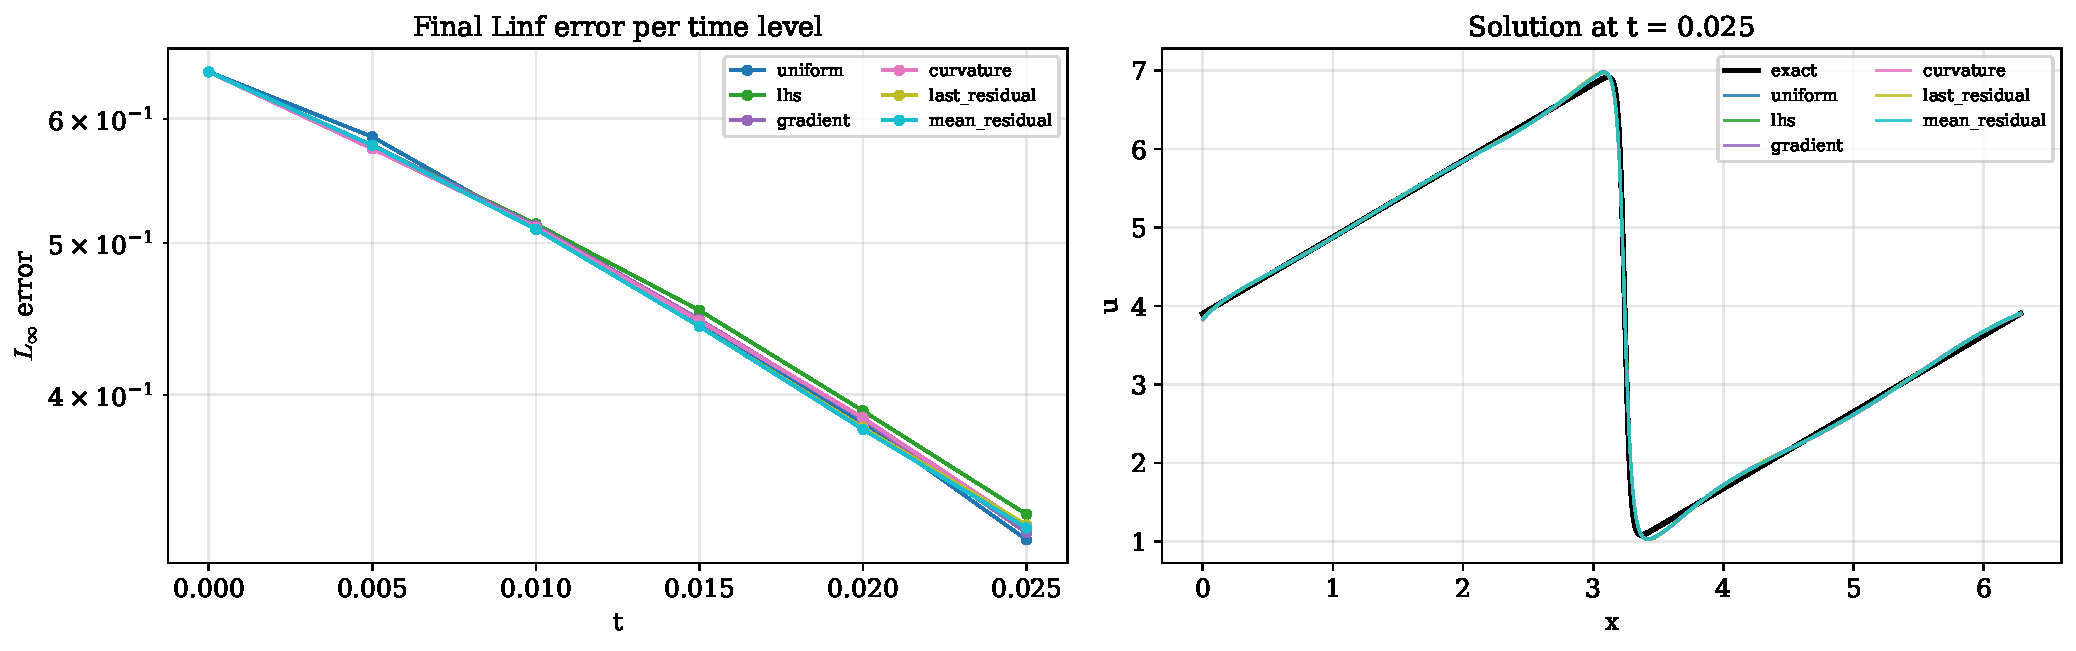
\includegraphics[width=\textwidth]{figs/collocation_burgers_solution_comparison_per_time.pdf}
  \caption{$L^\infty$ error per time level (left) and solution profiles at
    $t = 0.025$ (right) for all collocation strategies on the Burgers sawtooth
    benchmark.}
  \label{fig:colloc_burgers_sol}
\end{figure}

\begin{figure}[H]
  \centering
  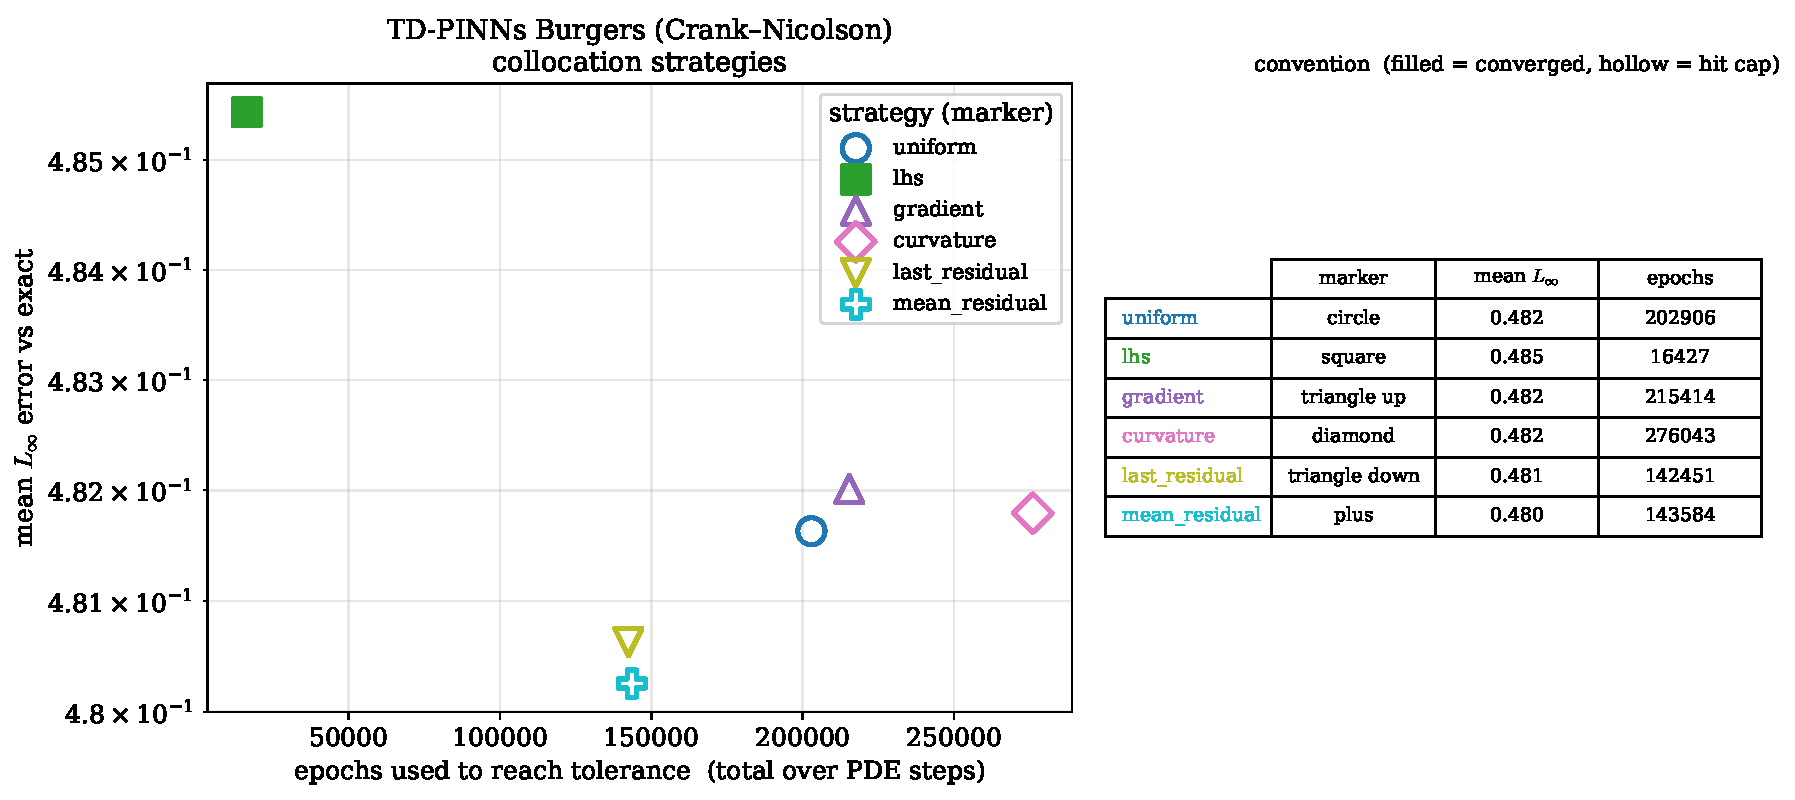
\includegraphics[width=0.75\textwidth]{figs/collocation_burgers_epochs_linf.pdf}
  \caption{Mean $L^1$ error versus total epoch count for all collocation
    strategies on the Burgers benchmark (Crank--Nicholson, $\nu = 0.07$).}
  \label{fig:colloc_burgers_epochs}
\end{figure}

% ─────────────────────────────────────────────────────────────────────────────
\section{Time-Integrator Comparison}
\label{sec:integrators}
% ─────────────────────────────────────────────────────────────────────────────

With the three schemes of Section~\ref{sec:bc} in hand---explicit Euler,
implicit (backward) Euler, and Crank--Nicholson---we now ask which one to march
the benchmark with. Each integrator is trained on the sawtooth case for a
\emph{fixed} epoch budget per step (no early stopping), and two quantities are
recorded: the training loss the optimiser reaches at the end of the budget, and
the $L^\infty$ error of the result against the Hopf--Cole analytic solution.

Figure~\ref{fig:integrator_loss} plots the two against each other, one point per
integrator: the horizontal axis is the training loss reached and the vertical
axis is the analytic $L^\infty$ error, so lower-left is better on both counts.
Crank--Nicholson attains the lowest true error. The subtlety is the horizontal
axis: in some runs implicit Euler ends at a \emph{lower training loss} than
Crank--Nicholson, which might suggest it is more accurate. It is not. The
training loss is the PDE residual the network is optimising---a self-referential
measure that the scheme grades against its own discretisation, not against the
exact solution---so a smaller training loss does not imply a smaller true error.
Measured against the analytic ground truth, Crank--Nicholson is consistently the
most accurate, with explicit Euler the least, as expected from its first-order,
conditionally stable nature.

\begin{figure}[H]
  \centering
  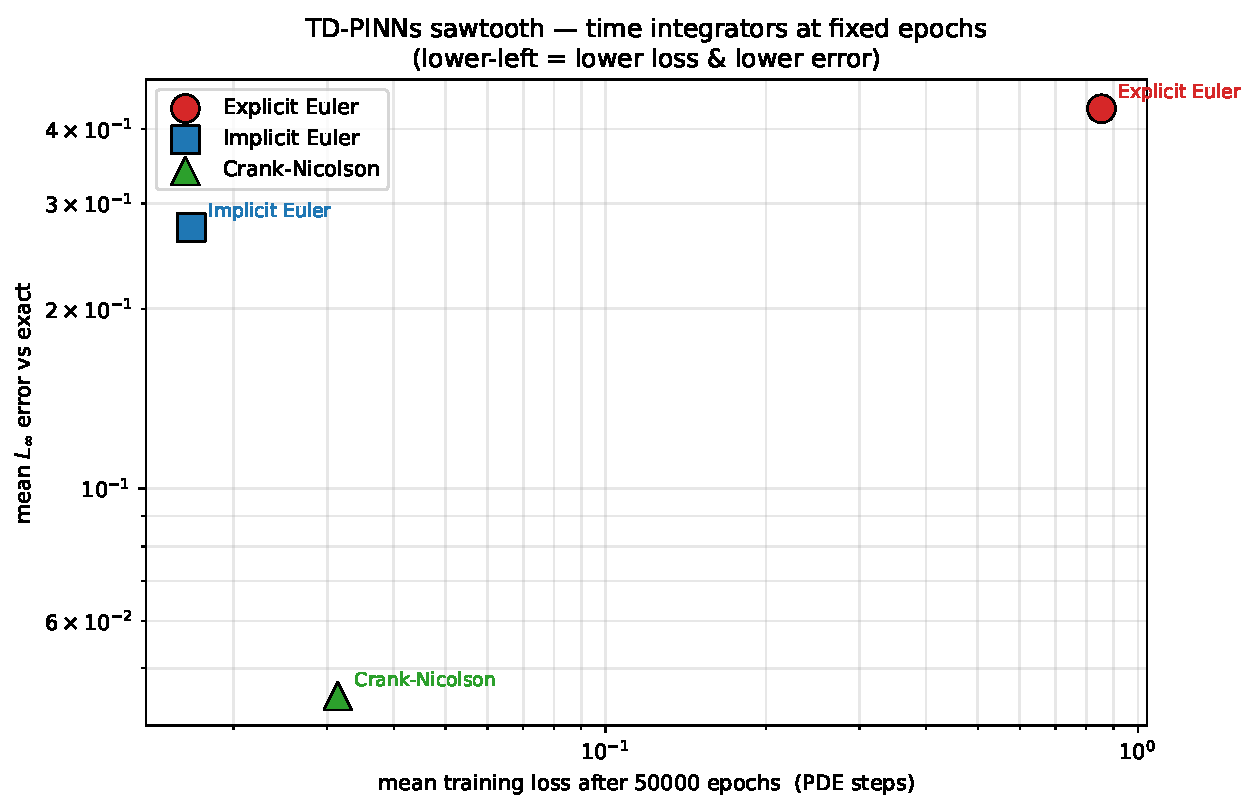
\includegraphics[width=0.75\textwidth]{figs/time_integrators_loss_vs_linf.pdf}
  \caption{Training loss reached versus analytic $L^\infty$ error at a fixed
    epoch budget, one point per time integrator on the Burgers sawtooth
    benchmark.}
  \label{fig:integrator_loss}
\end{figure}

The per-level errors and the solution profiles in
Figure~\ref{fig:integrator_errors} confirm the ranking against the true
solution: Crank--Nicholson tracks the analytic profile most closely across the
$L^1$, $L^2$, and $L^\infty$ norms, while implicit Euler's apparent advantage in
training loss does not carry over to the error against the exact solution. This
is why Crank--Nicholson is the scheme used for the method benchmark that
follows.

\begin{figure}[H]
  \centering
  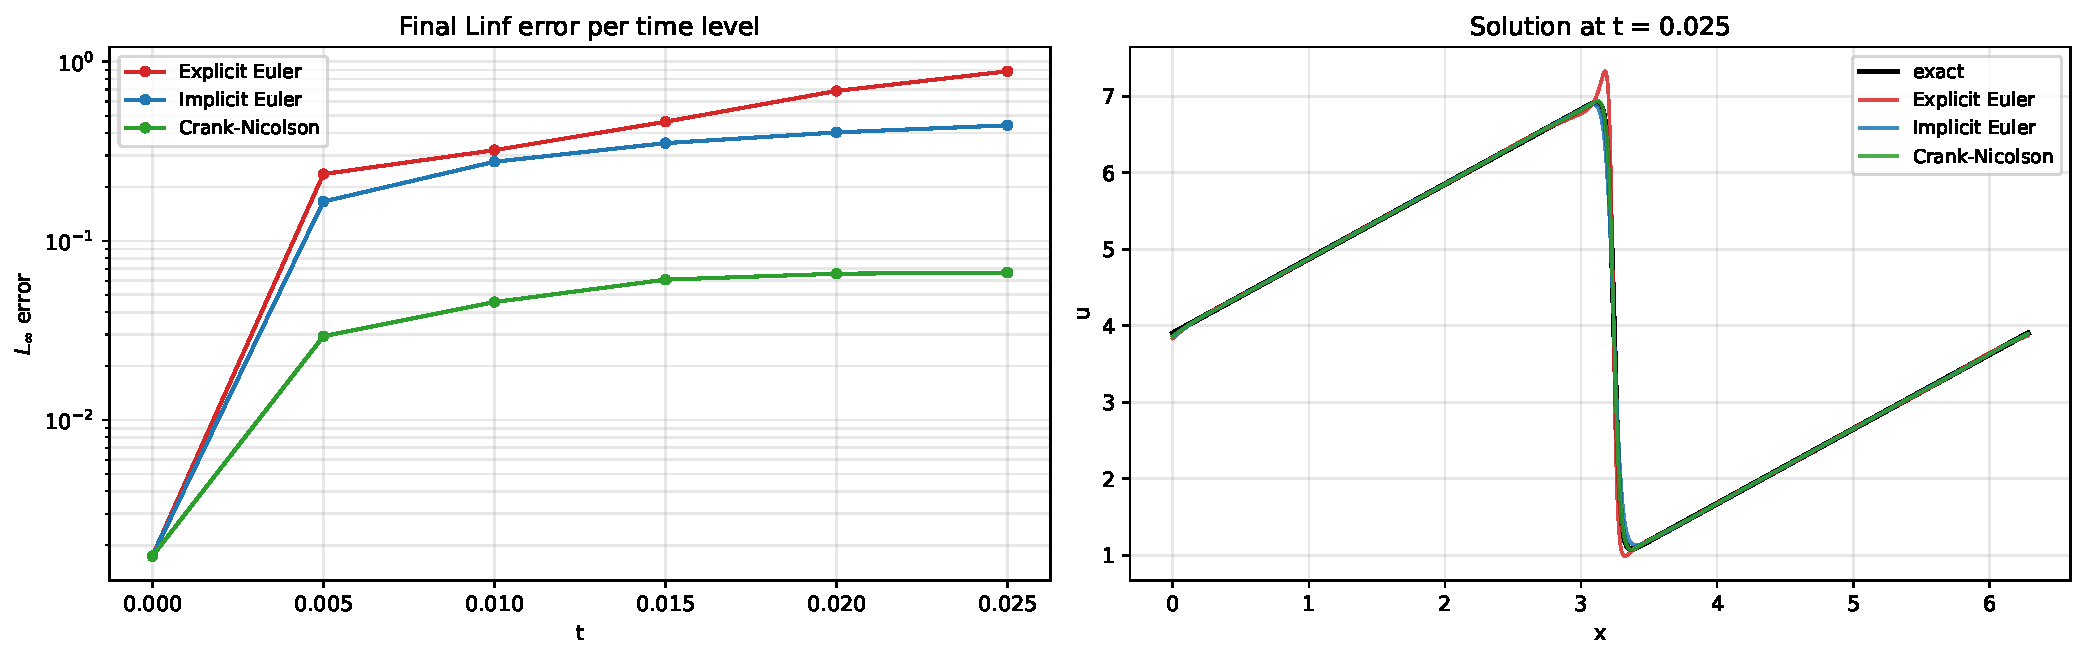
\includegraphics[width=\textwidth]{figs/time_integrators_loss_vs_linf_errors_and_solutons.pdf}
  \caption{Error norms per time level and solution profiles for explicit Euler,
    implicit Euler, and Crank--Nicholson against the Hopf--Cole analytic
    solution ($\nu = 0.07$, $T = 0.025$).}
  \label{fig:integrator_errors}
\end{figure}

% ─────────────────────────────────────────────────────────────────────────────
\section{Benchmark: TD-PINNs versus Vanilla PINN}
\label{sec:benchmark}
% ─────────────────────────────────────────────────────────────────────────────

The central comparison of the chapter pits the time-marching TD-PINN
(Crank--Nicholson) against a vanilla space--time PINN trained on the full
domain, both measured against the Hopf--Cole analytic solution. Three views
tell the story: the error growth in time, the pointwise solution at the final
step, and the conserved integrals.

Figure~\ref{fig:errors_vs_time} reports the $L^1$, $L^2$, and $L^\infty$ errors
at each time level. The TD-PINN starts roughly an order of magnitude more
accurate at $t = 0$---it fits the initial condition almost exactly---and then
accumulates error gradually as each step inherits the small approximation error
of its predecessor. The vanilla PINN, by contrast, holds a nearly flat error
profile across the window, reflecting its inability to resolve the temporal
structure of the solution. The $L^\infty$ norm is the most revealing: the
vanilla PINN sits near a constant ${\sim}5\times10^{-2}$ throughout, whereas the
TD-PINN climbs from ${\sim}4\times10^{-3}$ to ${\sim}6\times10^{-2}$ by
$t = 0.025$, finally meeting the vanilla curve. That crossover is the
signature of step-to-step error accumulation, and it identifies the principal
limitation of time-marching over long integration windows.

\begin{figure}[H]
  \centering
  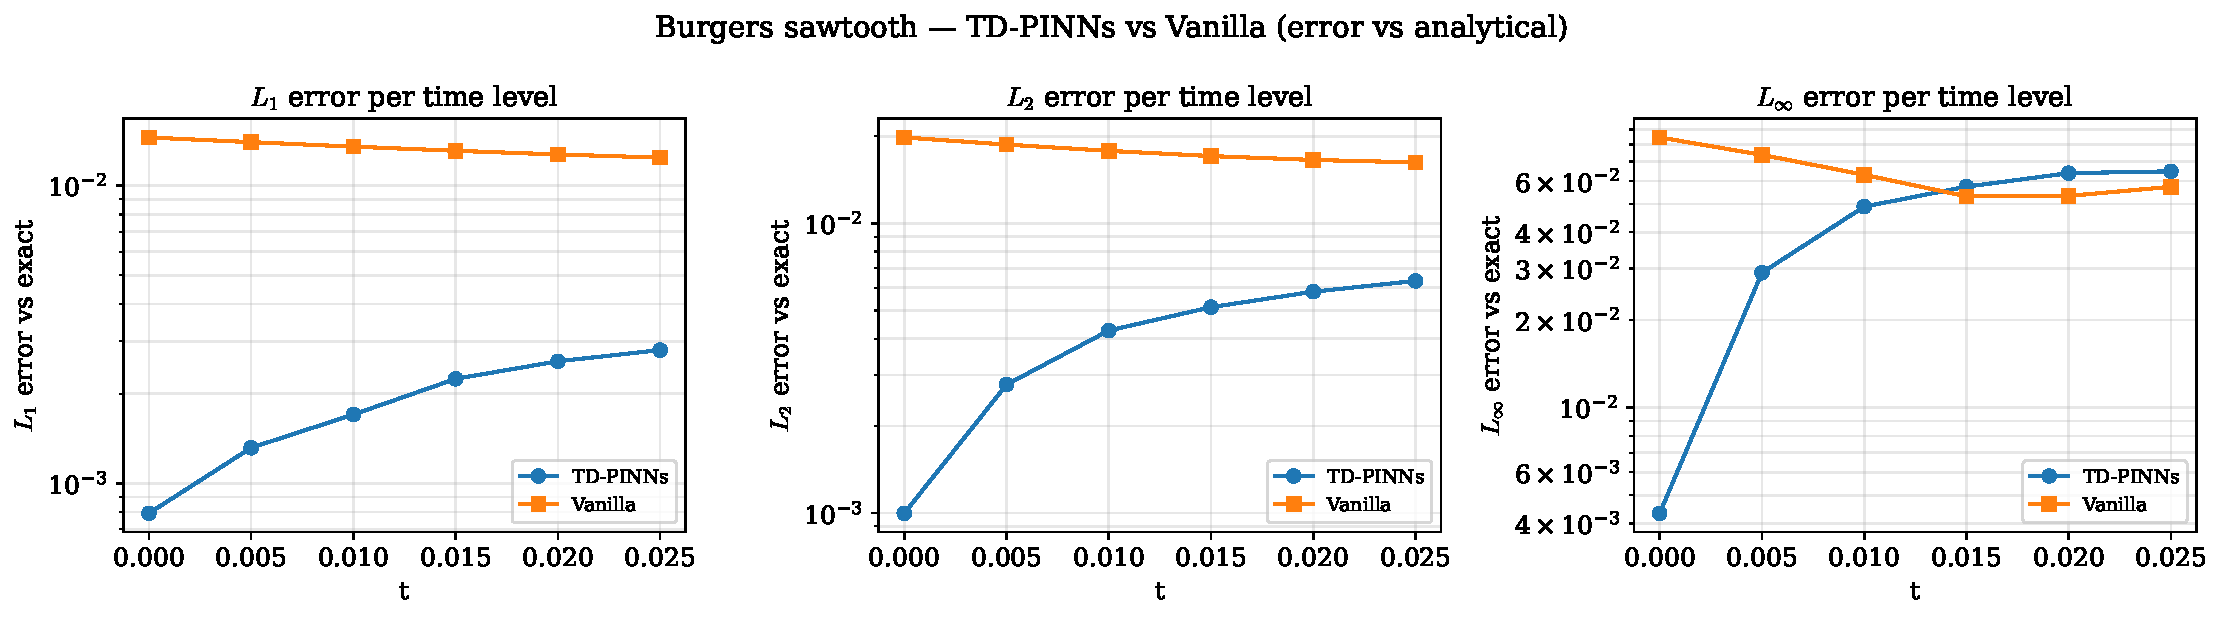
\includegraphics[width=\textwidth]{figs/burgers_methods_errors.pdf}
  \caption{$L^1$, $L^2$, and $L^\infty$ errors per time level: TD-PINNs
    (Crank--Nicholson) versus vanilla PINN against the Hopf--Cole solution
    ($\nu = 0.07$, $T = 0.025$).}
  \label{fig:errors_vs_time}
\end{figure}

The pointwise comparison at the final step (Figure~\ref{fig:solution_t025})
makes the crossover concrete. Both methods reproduce the sawtooth shape, but at
$t = 0.025$ the TD-PINN's peak error ($L^\infty = 6.47\times10^{-2}$) is now
slightly larger than the vanilla PINN's ($5.73\times10^{-2}$). In both cases
the error concentrates at the steep transition region, foreshadowing the
spectral-bias analysis of Section~\ref{sec:discussion}.

\begin{figure}[H]
  \centering
  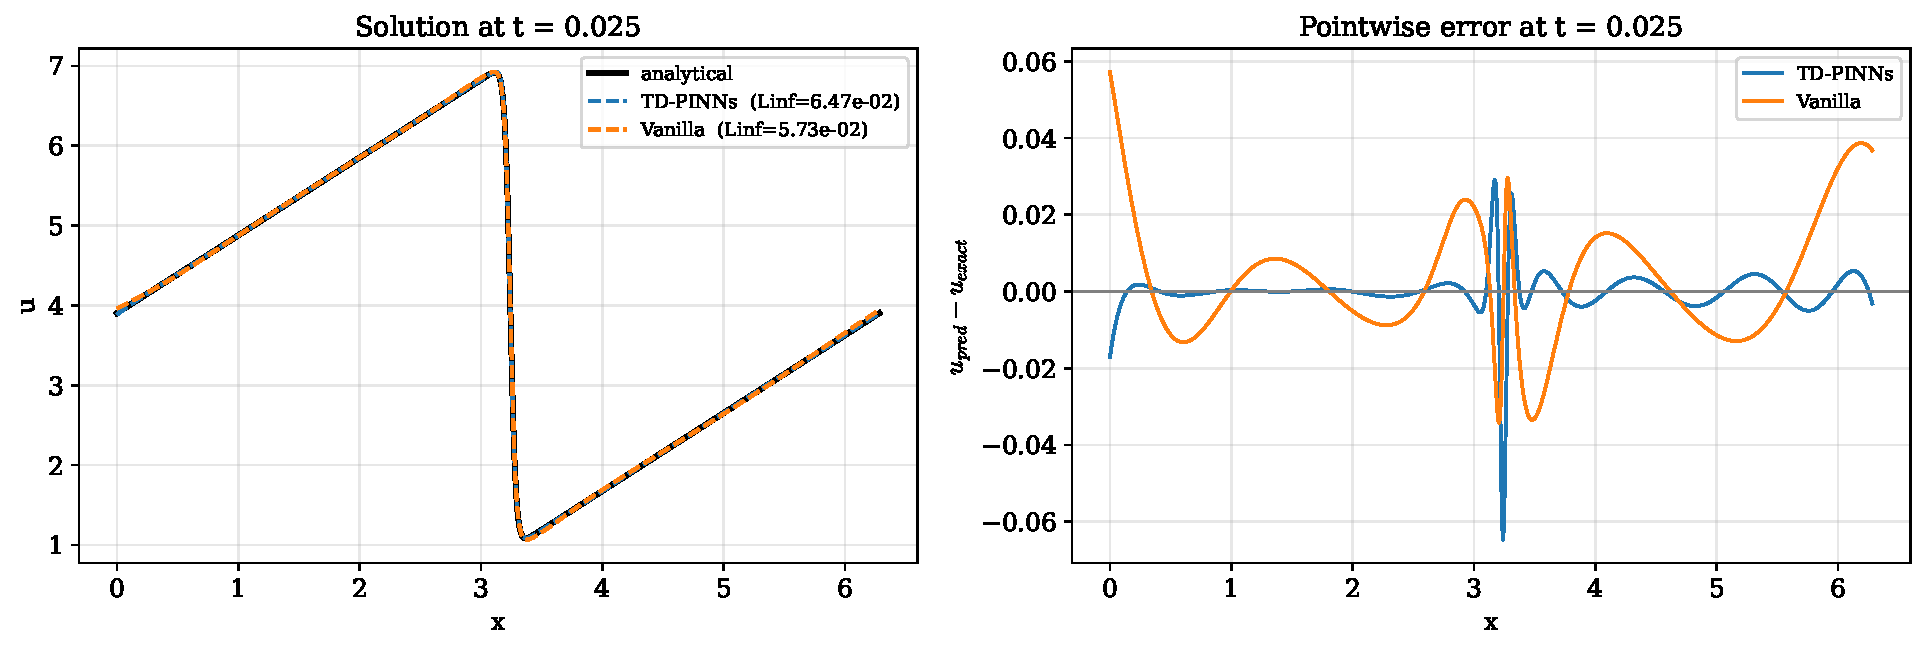
\includegraphics[width=0.82\textwidth]{figs/burgers_solution_t0p025.pdf}
  \caption{Solution (left) and pointwise error $\hat{u} - u_\text{exact}$
    (right) at $t = 0.025$ for TD-PINNs and vanilla PINN.}
  \label{fig:solution_t025}
\end{figure}

Finally, the conserved integrals in Figure~\ref{fig:conservation} test physical
consistency. Mass $\int u\,dx$ must stay constant and energy $\int u^2\,dx$ must
decrease monotonically under viscous dissipation ($dE/dt \leq 0$). The TD-PINN
conserves mass to within machine precision of the analytic value and tracks the
analytic dissipation rate closely, whereas the vanilla PINN shows a small but
systematic mass drift and under-dissipates energy at later times. The
time-marching scheme is thus not only more accurate early on but also more
faithful to the underlying conservation structure.

\begin{figure}[H]
  \centering
  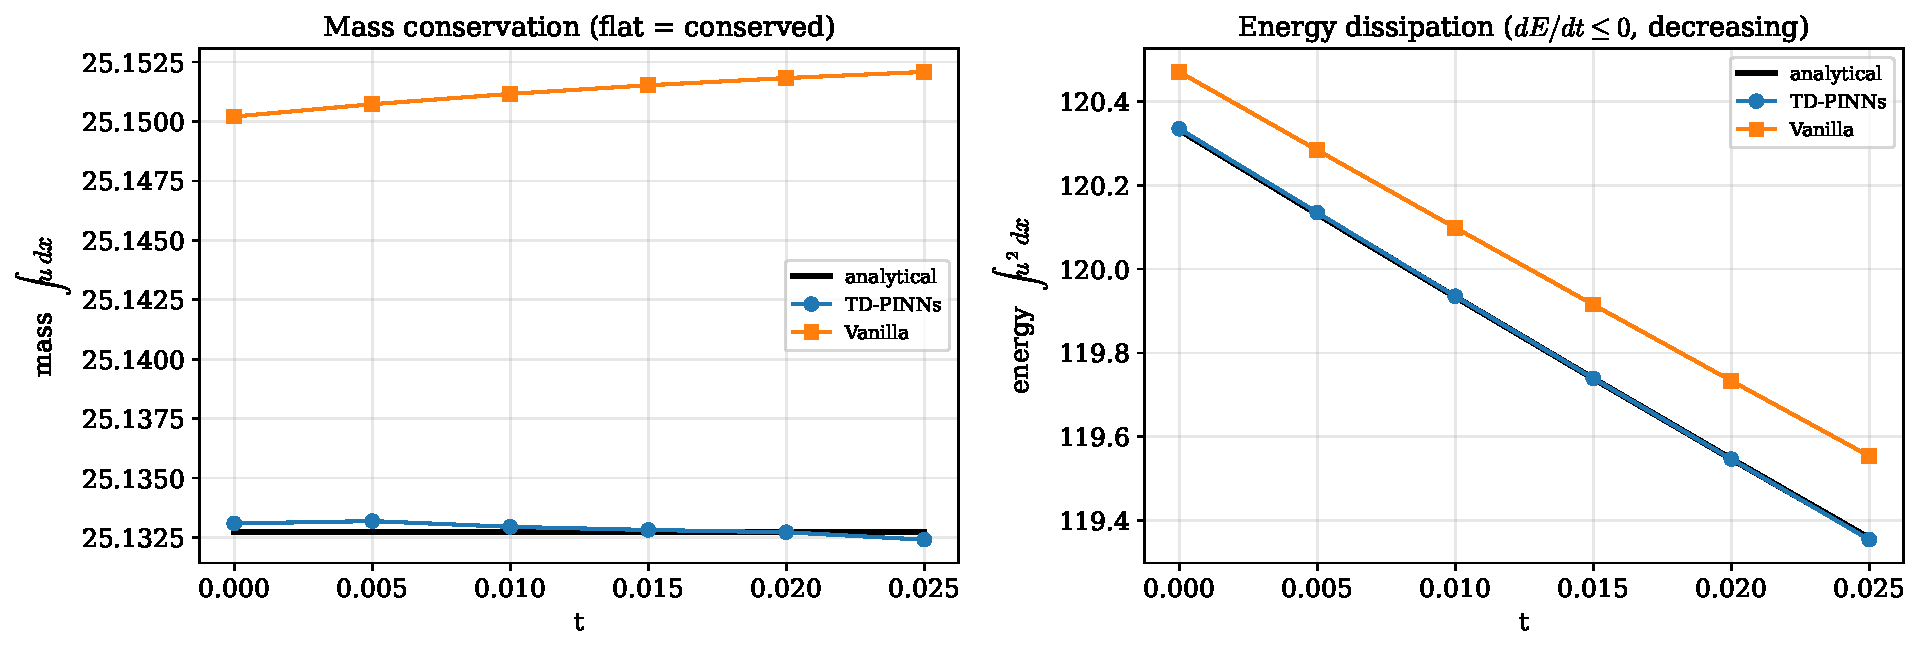
\includegraphics[width=\textwidth]{figs/burgers_methods_conservation.pdf}
  \caption{Mass $\int u\,dx$ (left) and energy $\int u^2\,dx$ (right) over time
    for TD-PINNs versus vanilla PINN.}
  \label{fig:conservation}
\end{figure}

% ─────────────────────────────────────────────────────────────────────────────
\section{Discussion}
\label{sec:discussion}
% ─────────────────────────────────────────────────────────────────────────────

The results above raise four threads worth following: the frequency structure
of the error, what makes a collocation criterion succeed, the practical cost of
the method, and its open limitations.

\subsection{Spectral Bias and Frequency-Resolved Error}

Networks with smooth activations exhibit spectral bias: gradient descent
preferentially reduces the loss carried by low-frequency Fourier modes and
leaves high-frequency components under-resolved~\cite{Rahaman2019}. To quantify
this, the predicted solution at the final step was transformed to the frequency
domain on a uniform periodic grid of $N = 512$ points,
\[
  \hat{u}_k = \frac{1}{N}\sum_{j=0}^{N-1} u(x_j)\,e^{-2\pi i kj/N},
  \qquad k = 0, 1, \ldots, \tfrac{N}{2},
\]
and the per-mode error $|\hat{u}_k^{\text{pred}} - \hat{u}_k^{\text{exact}}|$
was computed for both methods, then grouped into four bands: DC ($k=0$), low
($k = 1$--$4$), mid ($k = 5$--$15$), and high ($k \geq 16$).

The outcome is shown in Figure~\ref{fig:spectral_error}. Both methods reproduce
the magnitude spectrum well up to $k \approx 10$ and then fall short of the
analytic decay, with the gap widening into the high band. The per-mode error
stays below $10^{-4}$ for $k \leq 4$ and rises steeply thereafter; in the mid
band the TD-PINN is slightly more accurate, and by $k \approx 20$ the two
methods are comparable. Aggregated by band, the DC and low bands are
essentially exact for both, the mid band is where they differ most (in the
TD-PINN's favour), and the high band ($k \geq 16$) carries the bulk of the total
spectral error---direct confirmation that spectral bias is the dominant
limitation here.

\begin{figure}[H]
  \centering
  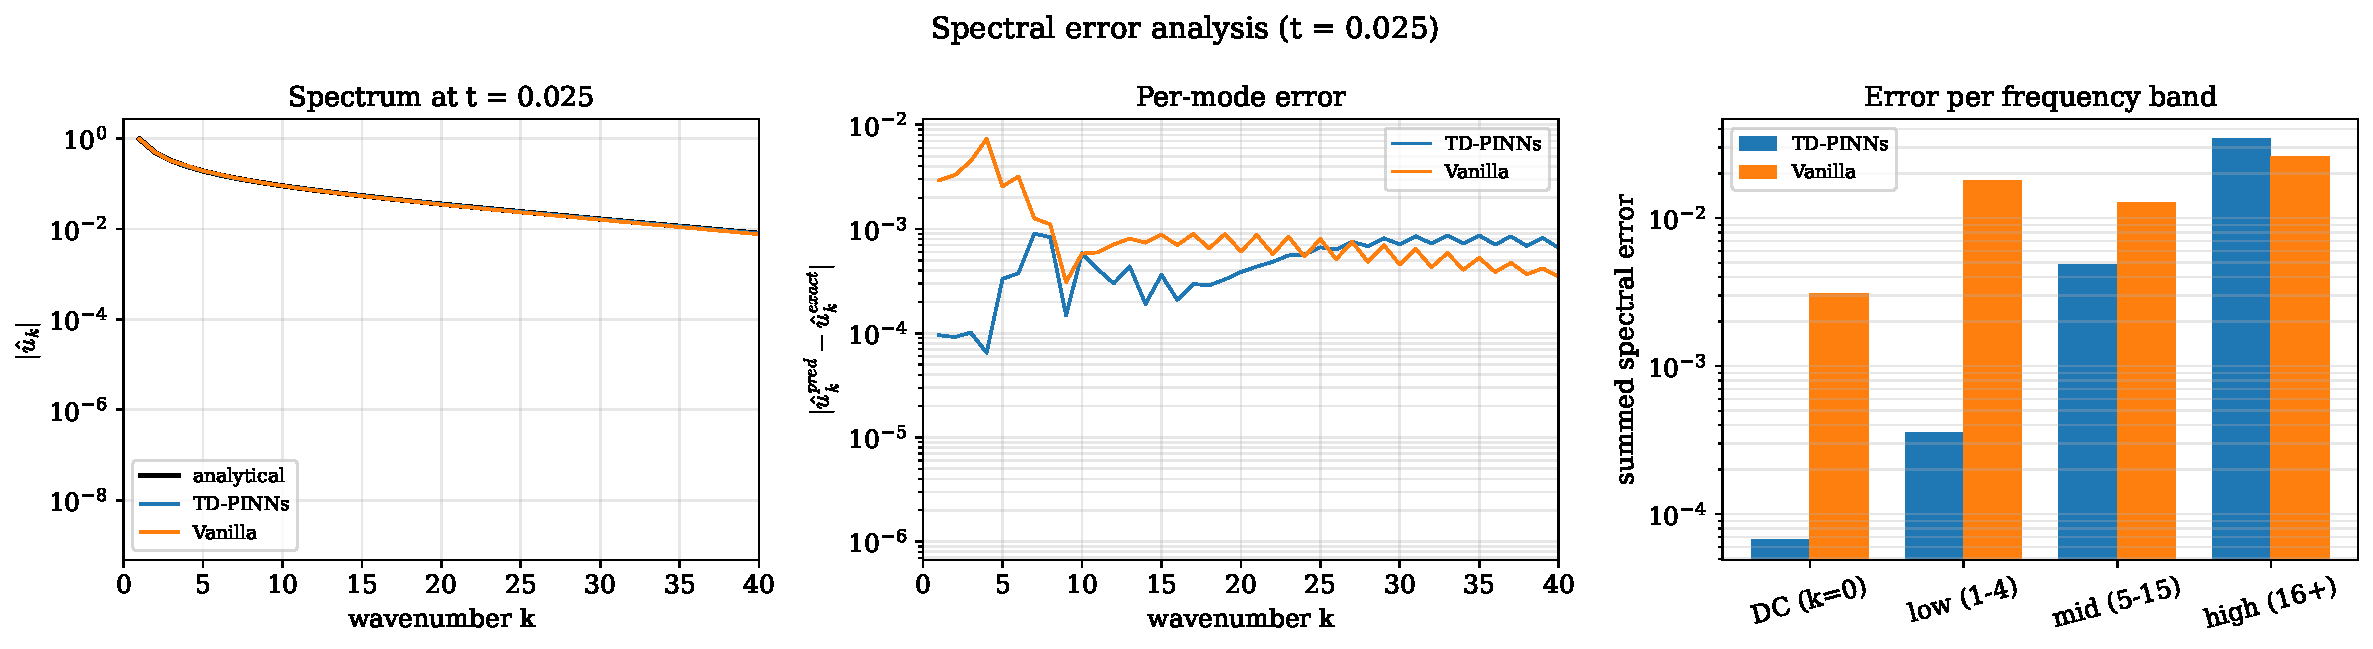
\includegraphics[width=\textwidth]{figs/burgers_methods_spectral.pdf}
  \caption{Spectral error at $t = 0.025$ ($\nu = 0.07$, $N = 512$):
    (a) magnitude spectrum $|\hat{u}_k|$;
    (b) per-mode error $|\hat{u}_k^\text{pred} - \hat{u}_k^\text{exact}|$;
    (c) summed error per frequency band.}
  \label{fig:spectral_error}
\end{figure}

\subsection{Collocation Strategy: Physics Alignment versus Direct Error Signal}

The contrasting diffusion and Burgers results point to a single principle. When
one operator dominates the solution, as diffusion does, a collocation criterion
derived from that operator (curvature) is optimal because it is algebraically
aligned with the PDE residual. When several operators compete nonlinearly, as
in Burgers, no geometric criterion reliably predicts where the \emph{next} step
will be hardest, and the residual-based strategy wins precisely because it
relies on a direct measurement of where the network was wrong rather than on an
assumption about operator dominance.

\begin{Rmk}{Practical recommendation}{rmk:colloc_rec}
  For smooth, diffusion-dominated problems, prefer curvature-based sampling: it
  mirrors the dominant PDE feature at minimal epoch cost. For nonlinear or
  multi-operator problems such as Burgers, residual-based sampling
  (\textit{mean\_residual}) is most accurate because it directly targets where
  the previous network erred. When the epoch budget is the binding constraint,
  LHS-1D offers the best accuracy--efficiency trade-off, matching residual
  accuracy at roughly $10\times$ fewer epochs.
\end{Rmk}

\subsection{Computational Considerations}

\paragraph{Transfer learning between steps.}
Because $u^t$ is generally close to $u^{t-1}$ for small $\Delta t$, warm-starting
the step-$t$ network from the step-$(t{-}1)$ weights markedly cuts the epochs
needed to converge. This temporal transfer learning was validated independently
in TL-DPINN~\cite{Chen2023}, where it reduced training time by up to $60\%$
without loss of accuracy.

\paragraph{Freezing gradients for Crank--Nicholson.}
The derivatives $\partial u^{t-1}/\partial x$ and
$\partial^2 u^{t-1}/\partial x^2$ required by scheme \eqref{eq:cn_scheme} are
computed once at the end of step $t-1$ and stored as fixed tensors, which
avoids redundant backpropagation through the old network at every iteration of
the current step.

\subsection{Limitations and Open Questions}

\begin{Rmk}{Arbitrary loss weights}{rmk:lossweights}
  As noted in Remark~\ref{rmk:weights}, the weights $\omega_\text{PDE}$,
  $\omega_\text{BC}$, and $\omega_\text{IC}$ do not live in a space with a
  natural metric~\cite{Wang2021}. Their magnitudes are problem-scale-dependent
  and their optimal values problem-specific, which keeps robust tuning an open
  challenge for soft-constraint PINNs~\cite{Sukumar2022}.
\end{Rmk}

\begin{Rmk}{Error accumulation across steps}{rmk:erroraccum}
  Each network $u^t$ introduces an approximation error that propagates as a
  frozen input to $u^{t+1}$. The $L^\infty$ crossover in
  Figure~\ref{fig:errors_vs_time} is the empirical signature of this
  accumulation: the TD-PINN starts below the vanilla PINN but drifts up to its
  level as steps pile up. Without adaptive step-size control or an a posteriori
  correction, this caps the practical integration window; the causal
  time-marching framework of Daw et al.~\cite{Daw2023} offers a principled
  remedy.
\end{Rmk}
